%% Journal of Intelligent Information Systems submission, built on the Springer Nature LaTeX template (sn-jnl.cls).
%% Numbers follow docs/research/Journal_Manuscript_Draft.md (v0.4) plus realdata/results (bootstrap, discovery,
%% full-log check).
\documentclass[pdflatex,sn-mathphys-num]{sn-jnl}

\usepackage{graphicx}
\usepackage{amsmath,amssymb}
\usepackage{booktabs}
\usepackage{url}
\usepackage{xcolor}
\usepackage{lineno}
\linenumbers

\begin{document}

\title[What Does Flattening Hide?]{What Does Flattening Hide? Measuring Case-Notion Distortion and Its Consequences on Seven Real Object-Centric Event Logs}

\author[1]{\fnm{Aakaash Sathya} \sur{Saravanan}}\email{aakaash.sathya2023@vitstudent.ac.in}
\equalcont{These authors contributed equally to this work.}
\author[1]{\fnm{Mitisha} \sur{Sharma}}\email{mitisha.sharma2023@vitstudent.ac.in}
\equalcont{These authors contributed equally to this work.}
\author[1]{\fnm{Tanmay} \sur{Khambete}}\email{tanmay.khambete2023@vitstudent.ac.in}
\equalcont{These authors contributed equally to this work.}
\author*[1]{\fnm{Kalyanaraman} \sur{P.}}\email{pkalyanaraman@vit.ac.in}

\affil[1]{\orgdiv{School of Computer Science and Engineering}, \orgname{Vellore Institute of Technology}, \orgaddress{\city{Vellore}, \postcode{632014}, \state{Tamil Nadu}, \country{India}}}

\abstract{Most process mining tools want exactly one case for each event. This is rarely how real information systems record data, since a single event often touches multiple objects. Analysts therefore flatten the data on one object type, so some events are duplicated and others are lost. This problem has been named before, but we have not seen it measured on real data. We measured it for seven public object-centric event logs (code review, education, legislation, e-mail, blockchain, software commits and a strategy game), 38 case notions in total. For each case notion we compared what an analyst would see in the flattened log with an object-centric reference. Three regimes emerged. Star logs do not lose or duplicate any events. In partitioned logs the median case notion loses 69\% to 91\% of the events. In fan-out logs a single event can become 81.65 rows. Duplication has little impact: only 2 case notions fall below an activity-rank correlation of 0.95 due to duplication alone. Narrowing is the larger issue. In 20 case notions most activities are missing from the flat log, and 2 of the 15 case notions that cover at least half of their log are among them. Discovered models do not show this, since every narrowed case notion still yields a model with replay fitness of 0.955 or more. Row counts from denormalised exports can reverse entity rankings (worst cases 0.16, \textminus0.01 and \textminus0.41). The headline numbers carry bootstrap intervals, and the pipeline reproduces them byte for byte.}

\keywords{Object-Centric Process Mining, OCEL 2.0, Event Data Flattening, Case Notion, Event Data Quality, Event Log Extraction}

\maketitle

\section{Introduction}\label{sec:intro}

Most process mining tools request a case identifier before they can analyse your data. This is easy to provide for a purchase order moving through three departments, but hard to provide for an e-mail. An e-mail has a sender, perhaps five recipients and a message identifier. A Gerrit code review can have a change, two reviewers and a project in one event.

In practice, people flatten the data. An object type is chosen as the case notion, and the log is then rewritten so that every event fits into exactly one case. Three issues can arise during this rewrite~\cite{vanderaalst2019ocpm}. An event containing several objects of the selected type is duplicated, once per object (convergence). An event with no object of the selected type is lost (deficiency). Repeated events that really belong to different objects of another type are merged into one case (divergence). Object-centric event logs have been designed so that they do not require this rewrite. Within OCEL~2.0~\cite{berti2024ocel20}, an event can refer to any number of typed objects, and objects can have relations with each other.

There are many reasons to believe that this additional structure matters. Convergence, divergence and deficiency have been handled within one approach~\cite{adams2024addressing}. One-to-many relationships produced directly-follows relations that did not really exist~\cite{waibel2022causal} in a case study at a food company. Machine-learning tasks perform better when the object graph is kept than when features are flattened~\cite{adams2023preserving}. Object-centric data also has quality issues of its own~\cite{kabierski2026quality}. In Moodle data, a student-centric view hides group and resource relations~\cite{miri2026educational}.

What we could not find were numbers. How often are events duplicated in a flattened view of real data, and how much is lost? Would an analyst viewing the resulting chart reach a different conclusion? Looking at Zenodo, 4TU and the wider web, we found worked examples and individual case studies, but no measurement that covered several real logs, although we cannot rule out having missed one. This article aims to provide that measurement. It makes three contributions.

\begin{enumerate}
\item Measurements of distortion metrics for seven real, public logs (38 case notions), which group the logs into three regimes.
\item A comparison of five common outputs between the flattened and object-centric views: activity rankings, directly-follows edges, variants, entity rankings and discovered models. Bootstrap intervals are included on the headline measurements. Throughout this work we keep duplication separate from narrowing, since duplication can be reversed by an analyst but narrowing cannot. We also separate narrowing in case notions that would plausibly be chosen from narrowing that is unavoidable because of how the log is structured.
\item Verification. A second implementation reproduces the distortion metrics exactly for all seven full logs, other independent checks cover other parts of the pipeline, and we report three bugs that these checks caught in our own code. One command reruns the entire study.
\end{enumerate}

There are also things this article does not claim. Object-centric logs have been used in education before~\cite{miri2026educational}, so that is not new. Nothing is claimed about how the processes of any particular organisation behave outside these seven logs, and seven logs are not enough to establish a general law.

\section{Background and related work}\label{sec:related}

\paragraph{The flattening problem.} Logs that allow one case per event misrepresent processes in which entities interact~\cite{vanderaalst2019ocpm}, and Adams and van der Aalst~\cite{adams2024addressing} have addressed convergence, deficiency and divergence together. Adams et al.~\cite{adams2022cases} have gone further by defining cases and variants directly on object-centric data, so that no case notion needs to be chosen. All this work is conceptual or algorithmic; none of it states how often the flattening effects occur in real logs. Recently, a research manifesto on object-centric process management~\cite{seidel2026manifesto} has been published. It aims to unify the terminology of object-centric modelling and mining, and it lists the open challenges of the field.

\paragraph{Format and extraction.} An OCEL~2.0 log~\cite{berti2024ocel20} contains events, objects, and the relationships between events and objects and between objects. Each relationship has a qualifier, and the log can be serialised as JSON, XML or SQLite. Extracting logs in this format from operational systems is a research topic in its own right. Berti et al.~\cite{berti2023sap} have extracted object-centric data from SAP ERP databases, and Egger et al.~\cite{egger2025unstructured} have brought unstructured data into object-centric process mining. Extraction determines which objects and relationships go into the log. Our question comes later: what is lost when this log is flattened for a tool that expects cases?

\paragraph{Consequences and quality.} Waibel et al.~\cite{waibel2022causal} have shown, using a causal event graph on one company's data, that one-to-many relationships cause spurious directly-follows relations. Kabierski et al.~\cite{kabierski2026quality} have created a classification of quality issues in object-centric data; they create a taxonomy of issues but do not state how often these issues occur. Adams et al.~\cite{adams2023preserving} have found that encodings that keep the object structure perform better than flattened features on predictive tasks.

\paragraph{Education and review processes.} Miri et al.~\cite{miri2026educational} have mined Moodle data using object-centric techniques, and Khayatbashi et al.~\cite{khayatbashi2026multidim} have extended object-centric process mining with multi-dimensional operations. Hassani et al.~\cite{hassani2018supervision} have reported on a department that oversees over 250 final-year computing projects, without event data. Premchaiswadi and Porouhan~\cite{premchaiswadi2015peer} have analysed an online peer-review process using one case notion. None of these studies measures flattening.

\section{Method}\label{sec:method}

\subsection{Logs and case notions}\label{sec:logs}

\paragraph{How the logs were chosen.} We started from academic project review, and there is no public event log of this process. We therefore began with two real logs of related processes, Gerrit code review (CROP~\cite{paixao2018crop}) and student enrolment and assessment (OULAD~\cite{kuzilek2017oulad}), and converted both into OCEL~2.0 ourselves. To see whether the results would hold outside these two domains, we looked for more logs on Zenodo, 4TU and the OCEL website. A log had to meet four conditions: it must record real activity, have an open licence, have timestamped events, and link events to at least two object types. Five logs met these conditions and were added. No simulated logs were included. A Moodle log with only one object type, an OpenReview corpus whose comments have no timestamps, and a publications log with no stated licence were also excluded. BPI Challenge 2019 was excluded because it is a flat log, and an OCEL would first have to be derived from it. The result is a purposive sample chosen for domain variety, not a random sample of object-centric logs.

Table~\ref{tab:logs} shows basic statistics. Five of the logs were already in OCEL format: Angular and Bundestag in JSON, Age of Empires in SQLite, and Enron and Ethereum as parquet bundles. The full Ethereum log has 3.2 million events, which is more than our 8\,GiB of memory can hold, so we work with a contiguous window of 300{,}000 events. In Enron, the e-mail addresses are hashed and separated by role into sender, recipient and copied. Each object type can be a \emph{case notion}. If its flat log has at least 1{,}000 events, we consider it \emph{analysed}; 38 case notions meet this criterion.

\begin{table}[htbp]
\caption{Seven logs. T -- Types of objects. O/E -- Number of objects per event. N -- Analysed case notions (at least 1{,}000 events)}\label{tab:logs}
\footnotesize
\setlength{\tabcolsep}{3pt}
\begin{tabular*}{\textwidth}{@{\extracolsep\fill}llrrrrr}
\toprule
Log & Domain & Events & Objects & T & O/E & N \\
\midrule
CROP (Gerrit) & Code Review & 306{,}716 & 55{,}323 & 3 & 3.0 & 3 \\
OULAD & Education & 216{,}532 & 61{,}577 & 4 & 3.8 & 4 \\
German Bundestag & Legislation & 62{,}719 & 37{,}665 & 44 & 1.1 & 9 \\
Age of Empires II & Game Play & 34{,}860 & 5{,}054 & 25 & 4.3 & 11 \\
Ethereum (Window) & Blockchain & 300{,}000 & 17{,}773 & 5 & 1.6 & 5 \\
Angular Commits & Software Commits & 27{,}842 & 28{,}317 & 2 & 88.0 & 2 \\
Enron Email & Email & 96{,}175 & 70{,}541 & 4 & 3.5 & 4 \\
\botrule
\end{tabular*}
\end{table}

\subsection{Distortion metrics}\label{sec:metrics}

Let $E$ be the set of events, $O$ the set of objects (object $o$ has type $\tau(o)$), and $R \subseteq E \times O$ the event-to-object relation. Let $T$ be a case notion. $R_T$ contains all pairs of $R$ whose object is of type $T$, and $E_T$ contains the events that occur in those pairs. Flattening on $T$ produces one row for each pair in $R_T$; this is also what the pm4py library does. The following were measured:

\begin{itemize}
\item \textbf{Deficiency} $\delta(T) = 1 - |E_T| / |E|$. This is the share of events lost in the flattened log; $1 - \delta(T)$ is the \emph{coverage} of $T$.
\item \textbf{Convergence share} $\kappa(T)$. This is the share of events in $E_T$ that have two or more $T$-objects.
\item \textbf{Copies per event} $c(T) = |R_T| / |E_T|$. This is 1.0 if no event is copied.
\item \textbf{Divergence share.} Take every combination of a case and an activity that occurs at least twice; the divergence share is the fraction of these whose events do not all have the same set of objects of some other type.
\item \textbf{Coupling.} For an ordered pair of types $(T, U)$, this is the share of $U$-objects that are included in events with two or more $T$-objects.
\end{itemize}

A type $U$ is a \emph{nested child} of type $T$ if at least 95\% of $U$'s objects are included in one $T$-case, each of these objects has its own lifecycle (two or more events), and on average there are at least 1.5 of them in a $T$-case. These three thresholds and the 1{,}000-event threshold have been chosen by us. In the code they are fixed at the top, and none has been changed to improve a result.

\subsection{Consequence analysis}\label{sec:consequence}

The object-centric view is used as the reference. Each event is counted once, and the directly-follows relation is built from consecutive events along the lifecycle of each object of every type. Each analysed case notion has been compared with this reference on four outputs. We also look at the model that an analyst would discover from the flattened log.

\begin{itemize}
\item \textbf{C1, activity ranking.} Spearman's $\rho$ has been calculated between the activity counts in the flattened log and (a)~the activity counts of the whole process and (b)~the counts of the same covered events, each counted once. Measure (b) shows the impact of duplication alone; measure (a) adds the impact of narrowing. We have also recorded the share of activities that can be seen at all. A case notion is \emph{narrowed} if less than half of the activities can be seen.
\item \textbf{C2, directly-follows edges.} How often event pairs are duplicated, and how similar the rankings of edge frequencies are with and without duplicates. If there are nested children, the spurious edge mass has also been calculated: the share of adjacent pairs in the flattened log whose edge type does not appear inside any child.
\item \textbf{C3, variants.} The number of distinct activity sequences per case.
\item \textbf{C4, entity ranking.} For every other type with at least 30 objects, we have correlated ($\rho$) the true number of events per object with the number of rows it would receive in a denormalised flat export of $T$, using the objects present in this export.
\item \textbf{C5, discovered model.} We have run the Inductive Miner with infrequent-behaviour filtering~\cite{leemans2014infrequent} (noise threshold 0.2) on every flattened log, using pm4py~\cite{berti2023pm4py}. For the resulting model we report token-based replay fitness~\cite{berti2019tbr}, token-based precision following Mu\~{n}oz-Gama and Carmona~\cite{munozgama2010precision}, the size of the process tree, its \emph{loop share} (the share of its visible activities that lie under a loop operator) and how many of the process's activities it contains. Precision has to replay every prefix of every case, so it becomes expensive. We have only calculated it if the sum of squared case lengths is at most $2 \times 10^7$, and each case notion was given at most one hour.
\end{itemize}

Ties in time are broken by the sorted event identifier, so the events are always in the same order.

\subsection{Plausible case notions and sensitivity}\label{sec:plausible}

Some object types would never be chosen as a case notion. In Age of Empires~II, a farm or a house is involved in only a few activities, and in the Bundestag log each object type is its own kind of parliamentary procedure. If such a case notion is narrowed, that follows from how the log is constructed. We wanted to distinguish this from narrowing that an analyst could reasonably walk into, so we looked at narrowing from two more angles. The \emph{widest} case notion in a log is the one that covers the most events; this is where most analysts would start. A case notion is \emph{plausible} if it covers half or more of the events in the log. These ideas were introduced after seeing the initial results. We have therefore reported the coverage threshold from 30\% to 70\%, the narrowing threshold from 0.3 to 0.7, and the event threshold raised from 1{,}000 to 2{,}000 and 5{,}000. The event threshold cannot be lowered without a new analysis, because case notions below it have never been analysed.

\subsection{Verification}\label{sec:verification}

We have done as much verification as possible. Every file downloaded from Zenodo is compared with its published size and MD5 and given a SHA-256 checksum. On a slice of 6{,}000 events from Enron (four case notions), a brute-force Python version of the directly-follows pairs and of one entity ranking gives the same answers as the vectorised code. Four rules from an earlier rule engine have been rewritten in SQL for CROP and give the same results, and three counts have been recalculated directly from the raw OULAD files. We also ran the full study again on a laptop, which took only a few minutes, and every tracked result file was byte-for-byte identical. During this process we discovered three bugs and resolved them: duplicate event rows within CROP (around 17\%), a missed Gerrit abandon message, and inconsistent event ordering where timestamps are equal. We also implemented a second version of the distortion metrics using basic dictionaries and sets; this version does not use pandas. It was run on the full versions of all seven logs and recomputed every metric in Section~\ref{sec:metrics}. It produced results identical to the published ones for all object types (87 case notions, including those below the threshold) and all 294 ordered type pairs. This check runs as part of the one-command build. We have not, however, found an independent labeller or had a second team review the converters.

\subsection{Uncertainty}\label{sec:uncertainty}

All numbers come from the complete data of each log. Therefore, the main source of uncertainty is which events and items each log happens to contain. The uncertainty was estimated from 200 bootstrap replicates with a fixed seed. The counts of case notions (narrowed, plausible, and both) were recalculated after weighting each event by a Poisson(1) draw, which changes coverage and activity visibility. Rank correlations need a different resampling unit: the ranked items are sampled with replacement, namely activities for C1 and visible entities for C4. Our initial attempt used event weighting here as well, and it went wrong: an entity with only one event receives the same weight in its true count and in its row count, which creates agreement that the data does not contain. The intervals run from the 2.5th to the 97.5th percentile. They capture the sampling noise within the seven logs, not the choice of logs. The unweighted replicate reproduces every published value.

\subsection{Generative AI}\label{sec:ai}

A large language model (Claude, from Anthropic) was used as an assistant. It helped write and review parts of the analysis, verification and figure-generation code, and it helped with drafting, rewriting and editing parts of the manuscript. The research question, the logs selected, the metrics and the interpretation were all decided by us. All numbers in the paper were generated by the released code from the public data. We have checked the code and its results, reviewed all text, and are fully responsible for the content.

\section{Results}\label{sec:results}

\subsection{Three regimes of distortion}\label{sec:regimes}

The distortion for each log is shown in Table~\ref{tab:distortion} and Fig.~\ref{fig:regimes}. Three groups can be seen.

\begin{table}[htbp]
\caption{Flattening distortion for each log. Dropped: Median proportion of events a case notion dropped. Copies: Median and maximum copies per event. Dup.: Case notions with over 5\% duplication. Shared: Type pairs where half or more of one type's objects participate in events with two or more objects from the other.}\label{tab:distortion}
\footnotesize
\setlength{\tabcolsep}{3pt}
\begin{tabular*}{\textwidth}{@{\extracolsep\fill}llrrrrr}
\toprule
Log & Regime & Dropped & Copies med. & Copies max & Dup. & Shared \\
\midrule
CROP (Gerrit) & star & 0.0\% & 1.00 & 1.00 & 0 of 3 & 4 of 6 \\
OULAD & star & 0.0\% & 1.00 & 1.00 & 0 of 4 & 7 of 12 \\
German Bundestag & partitioned & 90.8\% & 1.00 & 1.27 & 2 of 9 & 2 of 13 \\
Age of Empires II & partitioned & 86.3\% & 1.01 & 1.76 & 4 of 11 & 50 of 137 \\
Ethereum (window) & partitioned & 68.9\% & 1.04 & 1.09 & 2 of 5 & 10 of 20 \\
Angular commits & fan-out & 0.1\% & 44.06 & 81.65 & 2 of 2 & 2 of 2 \\
Enron e-mail & fan-out & 23.1\% & 1.29 & 2.11 & 2 of 4 & 8 of 12 \\
\botrule
\end{tabular*}
\end{table}

\paragraph{Star logs (CROP, OULAD).} There are no events in these logs that have two objects of the same type. As a result, nothing is copied (1.00 copies per event), and the median case notion loses no events. On these two measures the distortion is zero.

\paragraph{Partitioned logs (Bundestag, Age of Empires~II, Ethereum).} Again, there are relatively few copies. No case notion exceeds 1.27 copies per event in the Bundestag, 1.76 in Age of Empires~II or 1.09 in Ethereum. However, each object type covers a different part of the log. Therefore, the median case notion loses a lot of events: 69\% to 91\%.

\paragraph{Fan-out logs (Angular commits, Enron).} Here one event is related to many objects of the same type. As a result, duplication is high: up to 81.65 copies per event for the branch case notion in Angular, and 2.11 in Enron.

\begin{figure}[htbp]
\centering
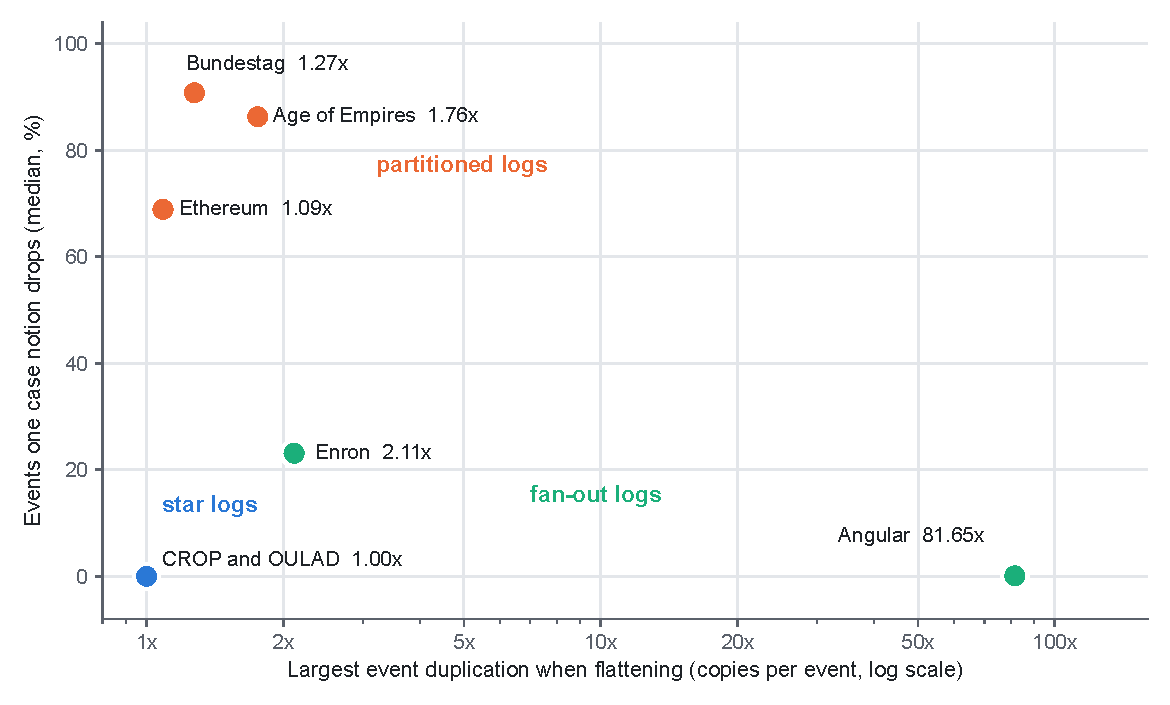
\includegraphics[width=0.85\textwidth]{Fig1}
\caption{Where each log sits on the two kinds of distortion (one dot per log). Horizontal: highest copies per event among its analysed case notions, on a log scale. Vertical: share of events lost by the median case notion}\label{fig:regimes}
\end{figure}

Coupling does not follow the three groups. Apart from the Bundestag (2 of 13 type pairs) and Age of Empires~II (50 of 137), at least half of the type pairs in every log are highly coupled, meaning that at least half of one type's objects are involved in events with two or more objects of the other type. In Angular, both pairs are highly coupled. The cases in these logs therefore overlap heavily, yet a flat view treats them as separate.

\subsection{Effects on common outputs}\label{sec:consequences}

\begin{table}[htbp]
\caption{Consequences of flattening per log. Visible: median share of activities visible. Act.~$\rho$: activity rank correlation against the whole process (median / lowest). Dup.~$\rho$: lowest activity rank correlation from duplication alone. Edge dup.: largest duplication of directly-follows pairs. Entity~$\rho$: lowest entity-rank correlation from a denormalised export}\label{tab:consequences}
\footnotesize
\setlength{\tabcolsep}{3pt}
\begin{tabular*}{\textwidth}{@{\extracolsep\fill}lrrrrrr}
\toprule
Log & Notions & Visible & Act.~$\rho$ & Dup.~$\rho$ & Edge dup. & Entity~$\rho$ \\
\midrule
CROP (Gerrit) & 3 & 1.00 & 1.00 / 1.00 & 1.00 & 1.00 & 1.00 \\
OULAD & 4 & 1.00 & 1.00 / 0.87 & 1.00 & 1.00 & 0.98 \\
German Bundestag & 9 & 0.10 & 0.17 / 0.00 & 1.00 & 1.26 & 0.34 \\
Age of Empires II & 11 & 0.12 & 0.21 / $-$0.05 & 1.00 & 1.69 & $-$0.41 \\
Ethereum (window) & 5 & 0.79 & 0.64 / 0.02 & 1.00 & 1.02 & $-$0.01 \\
Angular commits & 2 & 0.98 & 0.88 / 0.81 & 0.81 & 74.05 & 0.88 \\
Enron e-mail & 4 & 1.00 & 0.97 / 0.87 & 0.93 & 1.57 & 0.16 \\
\botrule
\end{tabular*}
\end{table}

\paragraph{Duplication alone rarely changes a ranking.} When the flat activity ranking is compared with a ranking in which each event appears only once, only 2 of the 38 case notions fall below $\rho = 0.95$ (bootstrap interval 1 to 3). These are the Angular files case notion at 0.81 (interval 0.66 to 0.90) and the Enron ``to'' role at 0.93. We have less confidence in the Enron value, as only nine activities are present, which makes its interval wide (0.53 to 1.00). Within both star logs, $\rho$ is exactly 1.0.

\paragraph{Narrowing is the larger effect, but much of it is structural.} In 20 of the 38 flat logs, more than half of the activities in the process do not appear. The median activity-rank correlation with the whole process is 0.17 (interval 0.14 to 0.29) for the Bundestag and 0.21 (0.15 to 0.29) for Age of Empires~II. Note that 18 of the 20 narrowed case notions come from these two logs. This is because certain object types, e.g.\ a written parliamentary question or a farm, are essentially sub-processes of their own; it is not surprising that a farm never sees the rest of the game. Both measures are plotted for all logs in Fig.~\ref{fig:activity}.

Restricting attention to plausible case notions (Section~\ref{sec:plausible}), we still see narrowing. There are 15 case notions that cover half or more of their log, and 2 of these are narrowed. For example, in Age of Empires~II the Villager case notion covers 52.8\% of the events but shows only 17\% of the activities. OULAD's Assessment case notion is the more interesting one. It covers 80\% of the events but shows only one activity out of three: all the submissions are there, but there are no registrations or withdrawals. More important to note is that two of the logs have no plausible case notion at all. The widest case notion covers 32.8\% of the events in the Bundestag and shows 3\% of its 148 activities, and in the Ethereum window it covers 37.4\%. Whatever object type an analyst chooses to investigate in these two logs, the flat view will be incomplete. The other five logs show very different results: their widest case notion covers ninety-five percent or more of the events and shows at least ninety-seven percent of the activities.

None of these figures depends on one threshold. With narrowing thresholds of 0.3, 0.4, 0.5, 0.6 and 0.7, there are 17, 18, 20, 20 and 20 narrowed case notions. With coverage thresholds of 30\%, 40\%, 50\%, 60\% and 70\%, there are 21, 16, 15, 13 and 13 plausible case notions, of which 5, 3, 2, 1 and 1 are narrowed; OULAD Assessment is narrowed at every threshold. If the event threshold is increased to 2{,}000, 33 case notions are left, of which 15 are narrowed; at 5{,}000, 28 are left and 10 are narrowed. Resampling does not affect the numbers either: in all 200 bootstrap replicates there are 20 narrowed case notions, 15 plausible ones and 2 that are both, as no case notion is close enough to a threshold to cross it.

\begin{figure}[htbp]
\centering
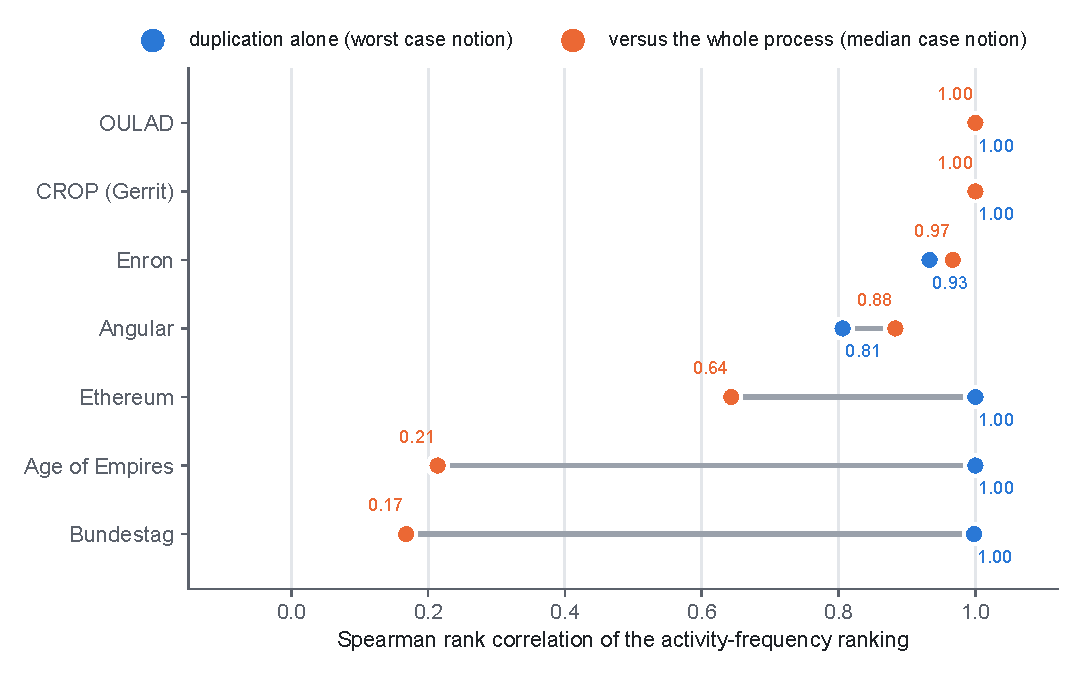
\includegraphics[width=0.85\textwidth]{Fig2}
\caption{The rank correlation between the flat activity ranking and the reference in each log. One point shows the worst case notion when duplication is the only effect; the other shows the median case notion against the whole process.}\label{fig:activity}
\end{figure}

\paragraph{Careless counting can mislead.} Imagine an analyst who ranks entities, such as people, by how many rows they have in a denormalised flat export. How accurate is this ranking? For the entities in the export (Fig.~\ref{fig:entity}), the worst case has a correlation of $\rho = 0.16$ in Enron (interval 0.14 to 0.18), $-0.01$ in Ethereum ($-0.03$ to 0.02) and $-0.41$ in Age of Empires~II ($-0.67$ to $-0.26$). None of these intervals reaches above 0.2. This problem can easily be solved by de-duplicating on the event identifier, so the result is a warning against counting rows rather than a loss that cannot be avoided.

\begin{figure}[htbp]
\centering
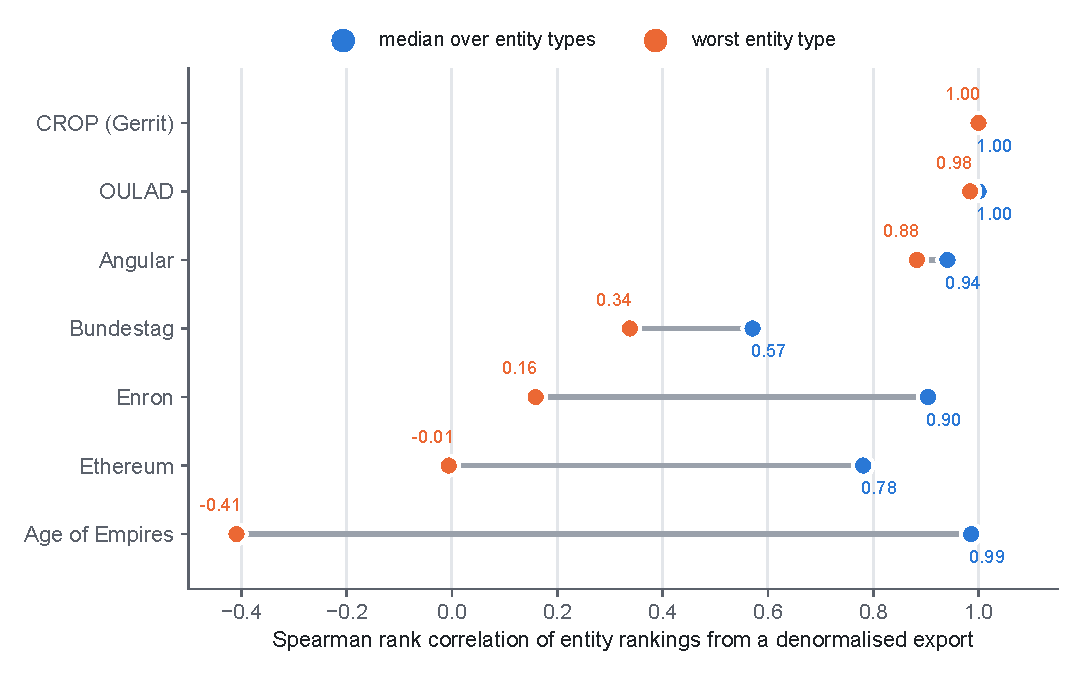
\includegraphics[width=0.85\textwidth]{Fig3}
\caption{Spearman's correlation between true events per entity and rows per entity in a denormalised flat export, using the median across entity types and worst entity type.}\label{fig:entity}
\end{figure}

\paragraph{Edges show a smaller effect.} Angular has the most duplicated directly-follows pairs, with 74 copies for the branch case notion. Where nested children are present, some flat edges connect two events that are unrelated in the data and adjacent only because flattening placed them next to each other. These spurious edges account for up to 27.7\% of adjacent pairs in Age of Empires~II and 16.6\% in OULAD.

\paragraph{A discovered model looks healthy even when it is partial.} Mining finished for 37 out of 38 case notions (Table~\ref{tab:discovery}). Only the branch case notion in Angular, with 2.27 million flat rows, could not be mined: it exceeded the one-hour time limit while its log was being replayed for fitness. In Age of Empires~II, Match and Session have only 10 and 20 cases respectively, with an average of about 3{,}500 and 1{,}700 events per case (the longest case has 8{,}895 events). Both first failed with a recursion error in pm4py's Inductive Miner while it simplifies the process tree; memory was not the issue, and both completed once we raised Python's recursion limit. The 37 models had a replay fitness between 0.955 and 1.000, with a median of 0.994, and all 20 narrowed case notions are among them. However, 20 of the models contain less than half of the activities in the process, and 12 contain less than 10\%. The fitness is calculated on the flat log that the model was mined from, so it cannot see what has been lost through flattening; a model with only 2\% of the activities scores as well as a complete model. The noise filter then removes a little more: 18 models lack activities that were present in the flat log. In Angular files, for example, the model has far fewer activities than the flat log (66\% of the activities in the model, compared to 97\% in the flat log).

\begin{table}[htbp]
\caption{Process Discovery results for the flat logs. (Inductive Miner, Noise threshold = 0.2). Mined = Case notions where the mining completed within the budget. Fitness = Lowest token based replay fitness. Precision = Median precision across case notions (number of case notions in brackets). Loops = Models where 90\% or more activities are in a loop. Partial = Models with less than half the activities in the process.}\label{tab:discovery}
\footnotesize
\setlength{\tabcolsep}{3pt}
\begin{tabular*}{\textwidth}{@{\extracolsep\fill}lrrrrr}
\toprule
Log & Mined & Fitness (min.) & Precision (med.) & Loops & Partial \\
\midrule
CROP (Gerrit) & 3 of 3 & 0.975 & 0.65 (1) & 3 & 0 \\
OULAD & 4 of 4 & 0.980 & 0.98 (2) & 3 & 1 \\
German Bundestag & 9 of 9 & 0.955 & 0.79 (9) & 1 & 9 \\
Age of Empires II & 11 of 11 & 0.977 & 0.30 (9) & 4 & 9 \\
Ethereum (window) & 5 of 5 & 0.979 & 0.07 (1) & 5 & 1 \\
Angular commits & 1 of 2 & 0.987 & 0.60 (1) & 0 & 0 \\
Enron e-mail & 4 of 4 & 0.984 & 0.99 (2) & 2 & 0 \\
\botrule
\end{tabular*}
\end{table}

\paragraph{Divergence turns into loops.} When a flat case contains repeated events that belong to different objects of another type, the miner will typically wrap them in a loop. Across the 37 case notions, the loop share increases with the divergence share (Spearman $\rho = 0.69$). In 14 of the 19 case notions with a divergence share of 0.5 or higher, 90\% or more of the activities are contained within a loop; among the remaining 18 case notions, this occurs in only 4. Precision, which we could calculate for 25 case notions, has a median of 0.67. The lowest 3 values (0.04 for the Player case notion of Age of Empires~II, 0.07 for Ethereum orders and 0.09 for Bundestag legislation) all come from models with 94\% or more of the activities in a loop. These models accept almost any order of events. As duplication increases, the models also grow and lose precision: tree size correlates with the number of copies per event at $\rho = 0.46$, and precision at $\rho = -0.57$ (25 case notions). With 37 case notions from 7 logs, we read these correlations as trends rather than laws.

\section{Discussion}\label{sec:discussion}

We expected to find mostly duplication, but this is not the case. Only two of the 7 logs had high duplication. What appears far more often is that a case notion does not cover much of the process, and the flat log does not give the analyst any indication of what is missing.

There is a lot of narrowing in the data, and much of it is structural, so an analyst familiar with the log would expect it: a case notion built for one kind of procedure will not give any insight into the other ones. Why measure it, then? There are two reasons. Firstly, analysts may not know how the log is structured, and in two of our 7 logs no object type covers even half of the events. Secondly, even case notions that look like sensible choices show narrowing. An analyst looking at the OULAD Assessment view would see 80\% of the events and assume that it is complete, yet would not be able to see a single withdrawal. Process discovery does not raise the alarm either. In our data, even a model created from a small part of the process still replays its own flat log almost perfectly, so it passes the usual quality check when it should not. If you take one habit from this article, we would like it to be this one: before trusting a flat result, ask which events and activities the case notion never saw.

This suggests three practical rules.

\begin{enumerate}
\item When presenting any flat result, state how much of the events and of the activities the case notion covers. These are two numbers to state, and they were the cheapest warning we found.
\item Remove duplicates based on the event identifier before counting anything, and count entities from the object-centric tables.
\item When objects of one type are shared between the cases of another (refer to the coupling figures), do not treat those cases as independent.
\end{enumerate}

\paragraph{Implications for information systems that log review processes.} An academic project portal is an example of an information system that logs a review process. A single action there can involve a project, a team, multiple students, a guide, a review stage and a version of the report. If such logs looked as we expect, flattening on the project would produce little duplication. However, it would hide the fact that one reviewer's effort is spread across many projects, which is the narrowing pattern, not the duplication pattern. We have not tested any data of this nature, so we make no claim about it; the obvious next step would be to test a de-identified portal log.

\section{Threats to validity}\label{sec:threats}

\begin{itemize}
\item \emph{Seven logs.} Whilst the domains vary, this is a purposive sample: the logs have been chosen for variety and availability, not randomly. The three regimes describe these logs, and we do not claim that they are the only ones.
\item \emph{Our choices.} We have chosen our case notions to be object types (and roles, for Enron), and we have chosen the nested-child thresholds and the 1{,}000-event cut-off. We decided to define a plausible case notion after seeing our initial results, which is why we report it across a range of thresholds; the conclusion holds across that range.
\item \emph{A window.} We have only used 300{,}000 of the 3.2 million events from Ethereum.
\item \emph{A data-quality flag.} Approximately 72 events in Enron (0.1\%) are dated before 1990, which is strange for a corpus from 1998 to 2002. We kept them.
\item \emph{Checking.} Our independent implementations are independent of the code they test, but they were written by the same team. Our second implementation of the distortion metrics now runs on the full logs. Our activity-ranking numbers, however, are only re-calculated by the bootstrap code, which loads the data in the same way as the analysis it checks. No second person labelled our findings, and our manual review of the classified CROP comments was performed by only one of us.
\item \emph{One miner.} C5 uses one discovery algorithm and one noise threshold. One of our 38 case notions (Angular branches) could not be mined within the time limit, and we could only calculate precision for 25. Other miners may well create different models.
\end{itemize}

\section{Conclusion}\label{sec:conclusion}

Overall, most of what flattening does to these logs is not duplication: only the 2 fan-out logs have high duplication. Narrowing is much more common; 20 of our 38 case notions show less than half of the activities in the process. Most of these are due to the structure of the log. However, 2 of the 15 case notions that cover half or more of their log are also narrowed, and in two logs no case notion reaches half of the events at all. Our usual checks do not pick this up. We still get a replay fitness of 0.955 or above from a model mined from a narrowed flat log, and divergence causes loops that let almost anything happen. Counting the rows in a denormalised export can even reverse an entity ranking. Our headline numbers hold under bootstrap resampling, one command re-runs our pipeline, and our distortion metrics have been confirmed on all 7 full logs by a second implementation. There is still work to do. The most valuable next step would be more real logs, ideally including one from an academic review portal, which is where this work started. We would also like someone from outside our team to label our findings, and we have only tried one discovery algorithm so far.

\backmatter

\bmhead{Acknowledgements}
We would like to thank Vellore Institute of Technology and its School of Computer Science and Engineering for the facilities and support that made this work possible. We would also like to thank the creators of the 7 public event logs for making their data available.

\section*{Statements and Declarations}

\begin{itemize}
\item \textbf{Funding.} No funding was received for conducting this study.
\item \textbf{Competing interests.} The authors have no relevant financial or non-financial interests to disclose.
\item \textbf{Ethics approval and consent to participate.} Not applicable. We only use public data with open licences. Personal identifiers in the Enron and CROP logs are hashed when loaded and never reported.
\item \textbf{Data availability.} All 7 logs are publicly available under a CC~BY~4.0 licence (OULAD as stated by its authors~\cite{kuzilek2017oulad}): CROP~\cite{data_crop}, OULAD~\cite{data_oulad}, German Bundestag~\cite{data_bundestag}, Age of Empires~II~\cite{data_aoe2}, Ethereum~\cite{data_ethereum}, Angular commits~\cite{data_angular} and Enron~\cite{data_enron}.
\item \textbf{Code availability.} Our code is publicly available at \url{https://github.com/ssaakaash/ocel-research}. It downloads and verifies our data and re-calculates all our numbers and figures. One command (\texttt{make study}) runs our main study and the full-log check, and a second (\texttt{make extended}) runs our bootstrap and the process-discovery comparison.
\item \textbf{Author contributions.} Aakaash Sathya Saravanan, Mitisha Sharma and Tanmay Khambete contributed equally to this work. Conceptualization, Methodology, Software, Validation, Formal analysis, Investigation, Data Curation, Visualization, Writing -- Original Draft: Aakaash Sathya Saravanan, Mitisha Sharma, Tanmay Khambete. Supervision, Writing -- Review \& Editing: Kalyanaraman P. All authors have read and approved the final manuscript.
\end{itemize}

\bibliography{refs}

\end{document}
